\chapter{Sample curricula}

This book is designed to cover two full semesters at undergraduate level, CSCI 3302 and CSCI 4302 at CU Boulder, or a single semester ``crash course'' at graduate level. There are multiple avenues that an instructor could take, each with their unique theme and a varying set of prerequisites on the students. 
 

\section{An introduction to autonomous \emph{mobile} robots}
This describes a possible one semester curriculum, which takes the students from the kinematics of a differential-wheel platform to SLAM. This curriculum is involved and requires a firm background in trigonometry, probability theory and linear algebra. This might be too ambitious for third-year Computer Science students, but fares well with Aerospace and Electrical Engineering students, who often have a stronger, and more applied, mathematical background. This curriculum is therefore also well suited as ``advanced class'', e.g. in the fourth year of a CS curriculum.

\subsection{Overview}
The curriculum is motivated by a maze-solving competition that is described in Section \ref{sec:ratslife}. Solving the game can be accomplished using a variety of algorithms ranging from wall following (which requires simple proportional control) to Depth-first Search on the maze to full SLAM. Here, the rules are designed such that creating a map of the environment leads to a competitive advantage on the long run.

\subsection{Materials}
The competition can be easily re-created using card board or LEGO bricks and any miniature, differential wheel platform that is equipped with a camera to recognize simple markers in the environment (which serve as landmarks for SLAM). The setup can also easily be simulated in a physics-based simulation environment, which allows scaling this curriculum to a large number of participants. The setup used at CU Boulder using the e-Puck robot and the Webots simulator is shown in Figure \ref{fig:ratslifereal}.

\begin{figure}[!htb]
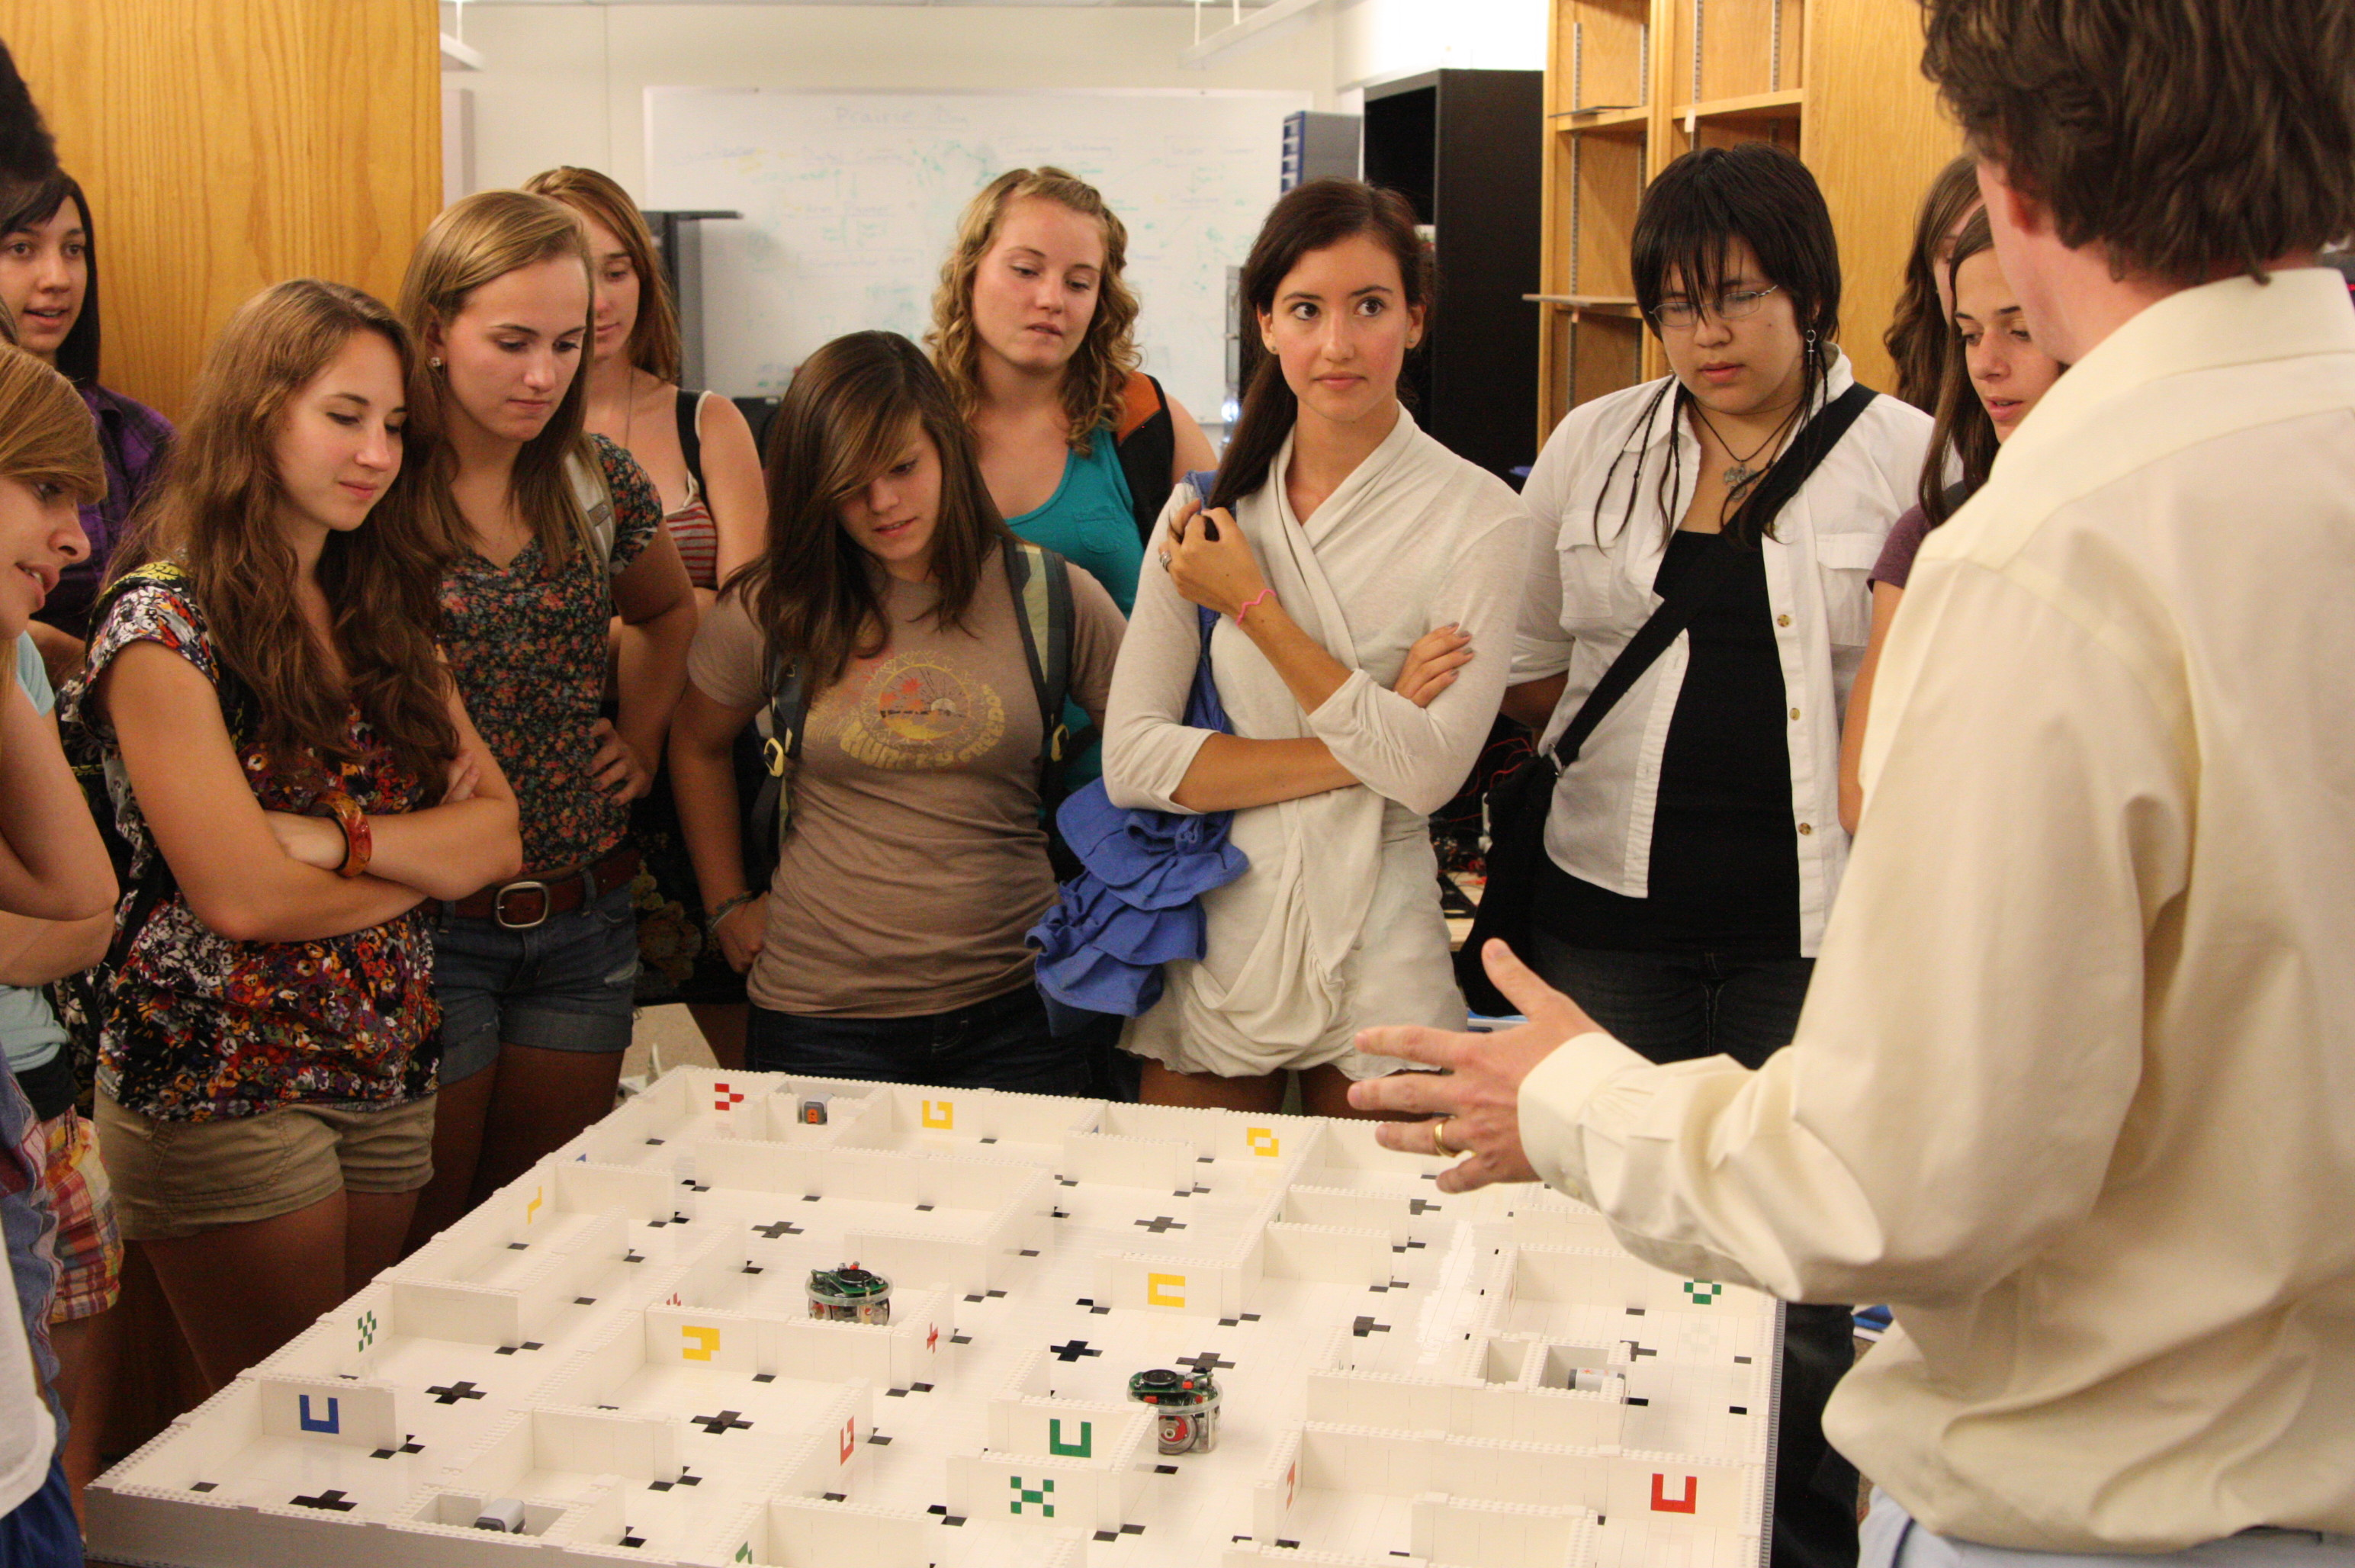
\includegraphics[width=0.48\textwidth]{figs/ratslife_real}
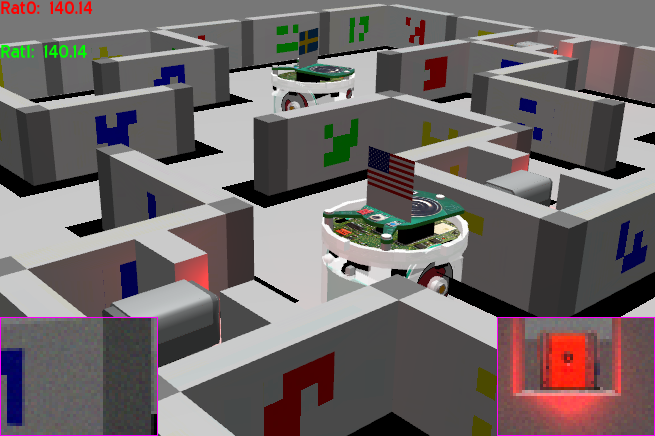
\includegraphics[width=0.48\textwidth]{figs/ratslife_webots}
\caption{\label{fig:ratslifereal}The ``Ratslife'' maze competition created from LEGO bricks and e-Puck robots (left). The same environment simulated in \emph{Webots}.}
\end{figure}

\subsection{Content}\label{sec:curr1content}
After introducing the field and the curriculum using Chapter \ref{chap:introduction} ``\nameref{chap:introduction}'', another week can be spend on basic concepts from Chapter \ref{chap:locomotion} ``\nameref{chap:locomotion}'', which includes concepts like ``\nameref{sec:stability}'' and ``\nameref{sec:dof}''. The lab portions of the class can at this time be used to introduce the software and hardware used in the competition. For example, students can experiment with the programming environment of the real robot or setup a simple world in the simulator themselves.

The lecture can then take up pace with Chapter \ref{chap:kinematics}. Here, the topics ``\nameref{sec:coordsystems}'', ``\nameref{sec:fwkmobile}'', and ``\nameref{sec:ivkmobile}'' are on the critical path, whereas other sections in Chapter \ref{chap:kinematics} are optional. It is worth mentioning that the forward kinematics of non-holonomic platforms, and in particular the motivation for considering their treatment in velocity rather than position space, are not straightforward and therefore at least some treatment of arm kinematics is recommended. These concepts can easily be turned into practical experience during the lab session. 

The ability to implement point-to-point motions in configuration space thanks to knowledge of inverse kinematics, directly lends itself to ``\nameref{sec:maps}'' and ``\nameref{chap:pathplanning}'' treated in Chapter \ref{chap:pathplanning}. For the purpose of maze solving, simple algorithms like Dijkstra's and A* are sufficient, and sampling-based approaches can be skipped. Implementing a path-planning algorithm both in simulation and on the real robot will provide first-hand experience of uncertainty. 

The lecture can then proceed to ``\nameref{chap:sensors}'' (Chapter \ref{chap:sensors}), which should be used to motivate uncertainty using concepts like accuracy and precision. These concepts can be formalized using materials in Chapter \ref{chap:statistics} ``\nameref{chap:statistics}'', and quantified during lab. Here, having students record the histogram of sensor noise distributions is a valuable exercise. 

Chapters \ref{chap:vision} and \ref{chap:feature_extraction}, which are on ``\nameref{chap:vision}'' and ``\nameref{chap:feature_extraction}'', do not need to extend further than needed to understand and implement simple algorithms for detecting the unique features in the maze environment. In practice, these can usually be detected using basic convolution-based filters from Chapter \ref{chap:vision}, and simple post-processing, introducing the notion of a ``feature'', but without reviewing more complex image feature detectors. The lab portion of the lab should be aimed at identifying markers in the environment, and can be scaffolded as much as necessary. 

Indepth experimentation with sensors, including vision, serves as a foundation for a more formal treatment of uncertainty in Chapter \ref{chap:uncertainty} ``\nameref{chap:uncertainty}''. Depending on whether the ``\nameref{sec:linefitting}'' example has been treated in Chapter \ref{chap:feature_extraction}, it can be used here to demonstrate error propagation from sensor uncertainty, and should be simplified otherwise. In lab, students can actually measure the distribution of robot position over hundreds of individual trials (this is an exercise that can be done collectively if enough hardware is available), and verify their math using these observations. Alternatively, code to perform these experiments can be provided, giving the students more time to catching up. 

The localization problem introduced in Chapter \ref{chap:localization} is best introduced using Markov localization, from which more advanced concepts such as the particle filter and the Kalman filter can be derived. Performing these experiments in the lab is involved, and are best done in simulation, which allows neat ways to visualize the probability distributions changing. 

The lecture can be concluded with ``\nameref{sec:ekfslam}'' in Chapter \ref{chap:slam}. Actually implementing EKF SLAM is beyond the scope of an undergraduate robotics class and is achieved only by very few students who go beyond the call of duty. Instead, students should be able to experience the workings of the algorithm in simulation, e.g., using one of the many available Matlab implementations, or scaffolded in the experimental platform by the instructor. 

The lab portion of the class can be concluded by a competition in which student teams compete against each other. In practice, winning teams differentiate themselves by the most rigorous implementation, often using one of the less complex algorithms, e.g., wall following or simple exploration. Here, it is up to the instructor incentivizing a desired approach. 

Depending on the pace of the class in lecture as well as the time that the instructor wishes to reserve for implementation of the final project, lectures can be offset by debates, as described in Section \ref{sec:debates}. 

\section{An introduction to autonomous manipulation}
Although robotic manipulation is a much less mature field than autonomous mobile robots, teaching its basics, such as those treated in this book, is slightly easier, mainly due to the fact that concepts like uncertainty and non-holonomy are mostly absent. Robotic manipulation is also well suited for a practice-based curriculum due to the wide array of cheap, multi-DOF robotic arms. These, of course, quickly reach their limitations to demonstrate advanced topics such as dynamics or force control, which are beyond the scope of this book.

\subsection{Overview} 
A manipulation-driven curriculum can be motivated by a ``grand challenge'' task such as robotic agriculture, robotic construction or assisted living, all of which have a manipulation problem at their core. Although a class project is likely to be limited to a toy-example, taking advantage of modern motion-planning frameworks and visualization tools, e.g. ROS/Moveit!, makes it easy to put the class into an industry-relevant framework and expose the students to state of the art platforms in simulation.

\subsection{Materials} 
Possible class project range from ``robot gardening'' or ``robots building robots'', for which setups can easily be created. These include real or plastic cherry tomato or strawberry plants and robotic construction kits such as Modular Robotics ``Cubelets'', which easily snap together and have the advantage to form structures that are robots themselves, adding additional motivation. The robot arm, such as the open-source, 7-DOF CLAM arm, can be mounted on a portable structure that contains fixed a set of fixed (3D) cameras. In order to allow a large number of students to get familiar with the necessary software and hardware, the instructor can provide a virtual machine with a preinstalled Linux environment and simulation tools. In particular, using the ``Robot Operating Systems'' (ROS) allows recording so-called ``bag''-files of sensor values, including entire sequences of joint recordings and RGB-D video. This allows the students to work on a large part of the homeworks and project preparation from a computer lab or from home, maximizing availability of real hardware.

\subsection{Content}
The first two weeks of this curriculum can be mostly identical to that described in Section \ref{sec:curr1content}. If a message passing system such as ROS is used, a good exercise is to record a histogram of message passing times in order to get familiar with the software.

In Chapter \ref{chap:kinematics}, the focus is instead on manipulating arms, including the Denavit-Hartenberg scheme and numerical methods for inverse kinematics. In turn, the topics ``\nameref{sec:fwkmobile}'', and ``\nameref{sec:ivkmobile}'' do not necessarily need to be included. Forward and inverse kinematics can be easily turned into lab sessions using Matlab/Mathematica, simulation or a real robot platform. If the class uses a more complex or industrial robot arm, an alternative path is to record joint trajectories in a ROS bag and letting the students explore this data, e.g., sketching 


\section{Class debates}\label{sec:debates}
Class debates are a good way to decompress at the end of class and require the students to put the materials they learned in a broader context. Student teams prepare pro and contra arguments for a statement of current technical or societal concern, exercising presentation and research skills. Sample topics include \emph{Robots putting humans out of work is a risk that needs to be mitigated}; \emph{Robots should not have the capability to autonomously discharge weapons / drive around in cities (autonomous cars)}; or \emph{Robots need to be made from components other than links, joints, and gears in order to reach the agility of people}.

The students are instructed to make as much use as possible of technical arguments that are grounded in the course materials and in additional literature. For example, students can use the inherent uncertainty of sensors to argue for or against enabling robots to use deadly weapons. Similarly, students relate the importance and impact of current developments in robotics to earlier inventions that led to industrialization, when considering the risk of robots putting humans out of work. 

Although suspicious as first, students usually receive this format very well.  While there is agreement that debates help to prepare them for the engineering profession by improving presentation skills, preparing engineers to think about questions posed by society, and reflecting up-to-date topics, the debates seem to have little effect on changing the students' actual opinions on a topic. For example, in a questionnaire administered after class, only two students responded positively. Students are also undecided about whether the debates helped them to better understand the technical content of the class. Yet students find the debate concept important enough that they prefer it over a more in-depth treatment of the technical content of the class, and disagree that debates should be given less time in class. However, students are undecided whether debates are important enough to merit early inclusion in the curriculum or to be part of every class in engineering. 

Concerning the overall format, students find that discussion time was too short when allotting 10 minutes per position and 15 minutes for discussion and rebuttal. Also, students tend to agree that debates are an opportunity to decompress (``relaxing''), which is desirable as this period of class coincides with wrapping up the course project.